
\documentclass[aspectratio=169,10pt,english]{beamer} 
\usepackage[utf8]{inputenc} 

\usepackage{beamer}

\usepackage{booktabs}
\usepackage{graphicx}
\usepackage{csquotes}
\usepackage{pdfpages}
\usepackage{gensymb}
\usepackage{hyperref}
\usepackage{tabto}

\title{\textbf{Depicting Uncertainty in 2.5D Treemaps}\enspace{}|\enspace{}VINCI 2020}
\subtitle{\underline{Daniel Limberger}, Matthias Trapp, and Jürgen Döllner.}
\author{Hasso Plattner Institute, University of Potsdam}

\newcommand{\websource}[1]{\footnote[frame]{\href{#1}{#1}}}

\newcommand\barefootnotetext[1]{%
  \begingroup
  \renewcommand\thefootnote{}\footnote{#1}%
  \addtocounter{footnote}{-1}%
  \endgroup
}

\begin{document} 

\begin{frame}[plain]
	
	\vspace{1.6cm}
	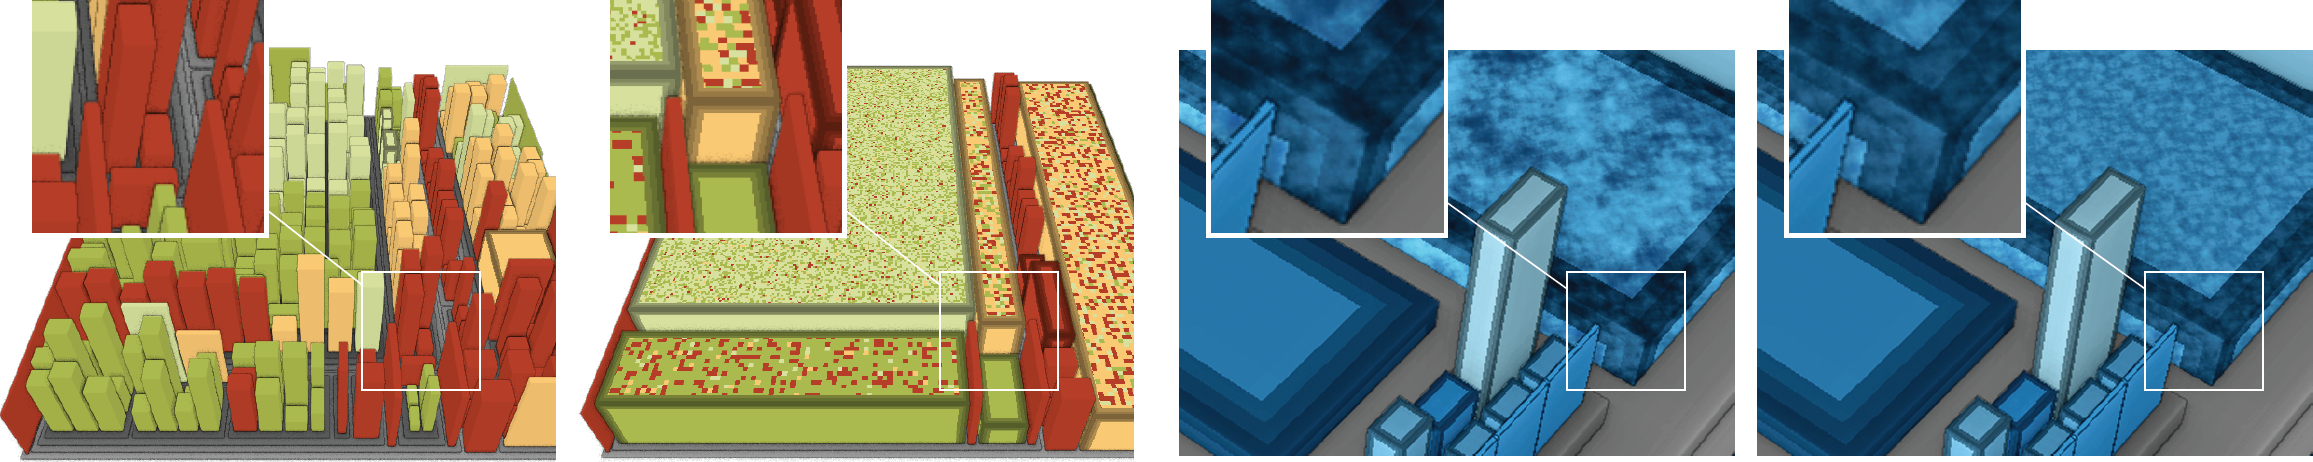
\includegraphics[width=\textwidth]{images/teaser-v1}
	\vspace{2.2cm}

	\titlepage
	
\end{frame} 

\begin{frame}[t]{Truth in Visualization}

    \bigskip

    \Large\emph{\enquote{[\ldots] what is \textbf{not} surrounded by uncertainty cannot be the truth.}}\\\smallskip
    \normalsize \hfill Richard Feynman --- Letter to the editor of the California Tech, 1976, in the context of physics.

    \bigskip
    \bigskip
    \bigskip
    \pause

    In order to be more truthful in visualization we need to account for uncertainty.
    \bigskip

    Robert B. Haber and David A. McNabb defined two types of uncertainty w.r.t. visualization:\\%~\cite{Haber1990}:\\
    The \textbf{visualization of uncertainty} and \textbf{uncertainty of visualization}.

\end{frame} 

\begin{frame}[t]{Uncertainty in Visualization}

    \begin{columns}[T,onlytextwidth]

        \column{0.42\textwidth}
    
        \textbf{Uncertainty in Data}
        \begin{itemize}
            \item accuracy of measurements
            \item biases within the data or data model
            \item probability of trend forecasts
            \item completeness of data
            \item confidence, variability, sampling, \ldots
        \end{itemize}

        \column{0.54\textwidth}

	    \textbf{Uncertainty in Visual Display and Perception}
        \begin{itemize}
            \item relevance of data w.r.t. task
            \item validity of measurements or data
            \item correctness of assumptions on data
            \item accuracy of visual variables
            \item display of accumulated data
        \end{itemize}
    	
    \end{columns}
    
    \bigskip
    \pause
    
    Uncertainty can only be mitigated to a certain extent and is highly use-case specific.
    \medskip
    
    In Visual Software Analytics:

    \begin{itemize}
        \item Most metrics, especially compound metrics, such as effort, code smells etc. carry an underlying assumption which can be easily missed when reading the visualization.
        \item In order to facilitate knowledge-based decision making or guiding, the visualization should provide information on the relevance of any data item.    
    \end{itemize}

\end{frame} 

\begin{frame}[t]{Uncertainty in Software Maps\enspace{}|\enspace{}\textbf{Attribute Uncertainty}}

    \begin{columns}[T,onlytextwidth]

        \column{0.54\textwidth}
    
        \textbf{Example:} Development activity within a software project using the number of modified lines-of-code:\medskip

        \begin{itemize}
            \item Mapping: Number of developers is mapped to color: red = 1, gray = 2, green > 2, height is LoC.
            \item Task: Identification of knowledge monopolies. %
        \end{itemize}

        \column{0.44\textwidth}

	    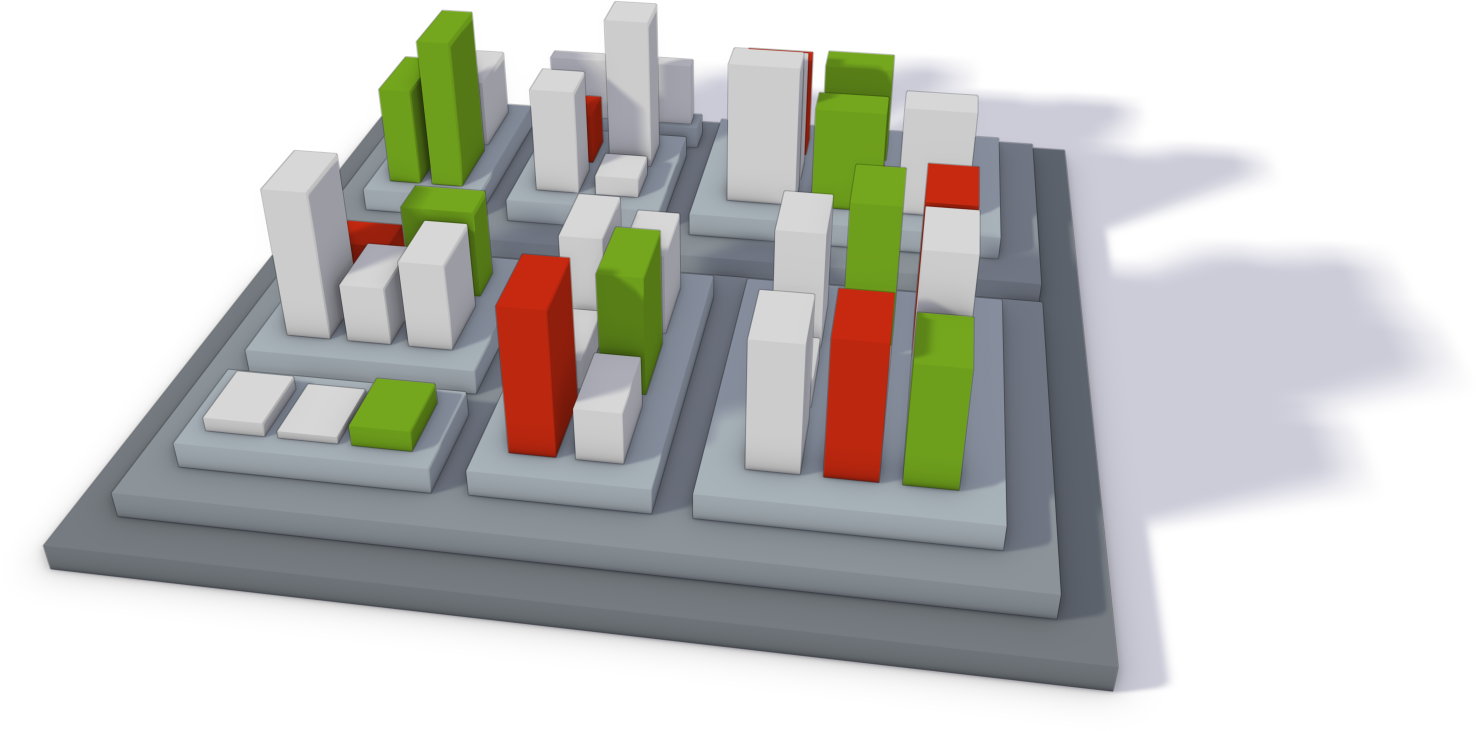
\includegraphics[width=\textwidth]{images/app-maps}
    	
    \end{columns}
    
    \textbf{Mind the Map:}

    \begin{itemize}
        \item Multiple cases where knowledge monopoly is missed, e.g., changes in non-overlapping parts, relevance of changes (e.g., fixing a typo, increment copy right year in the comments, duplicating code from other authors), etc.
        \item Is the mapping comparable with the same attributes mapped to other, similar software projects.
        \item[-] Comparability of attributes: normalization of metrics.
        \item[-] Comparability of visual variables: scale and intensity of height and color respectively.
    \end{itemize}
    
\end{frame}

\begin{frame}[t]{Uncertainty in Software Maps\enspace{}|\enspace{}\textbf{Distribution Uncertainty}}

    \medskip
    
    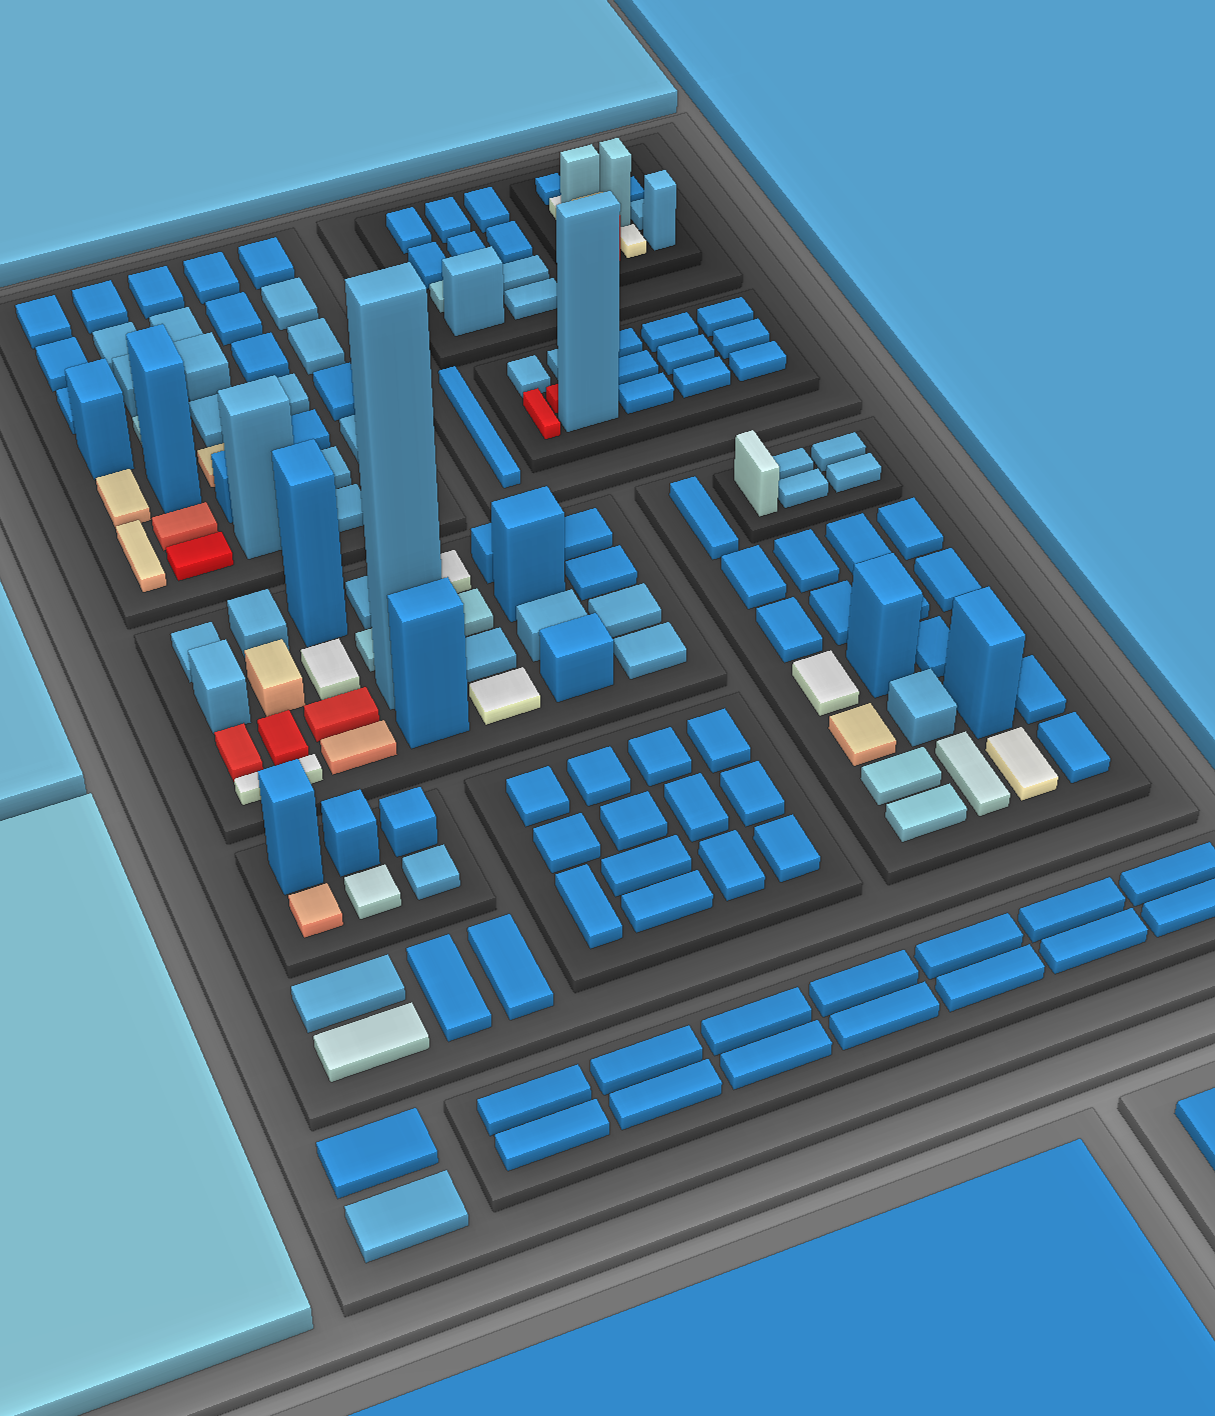
\includegraphics[height=3.5cm]{images/aggregated-0.png}
    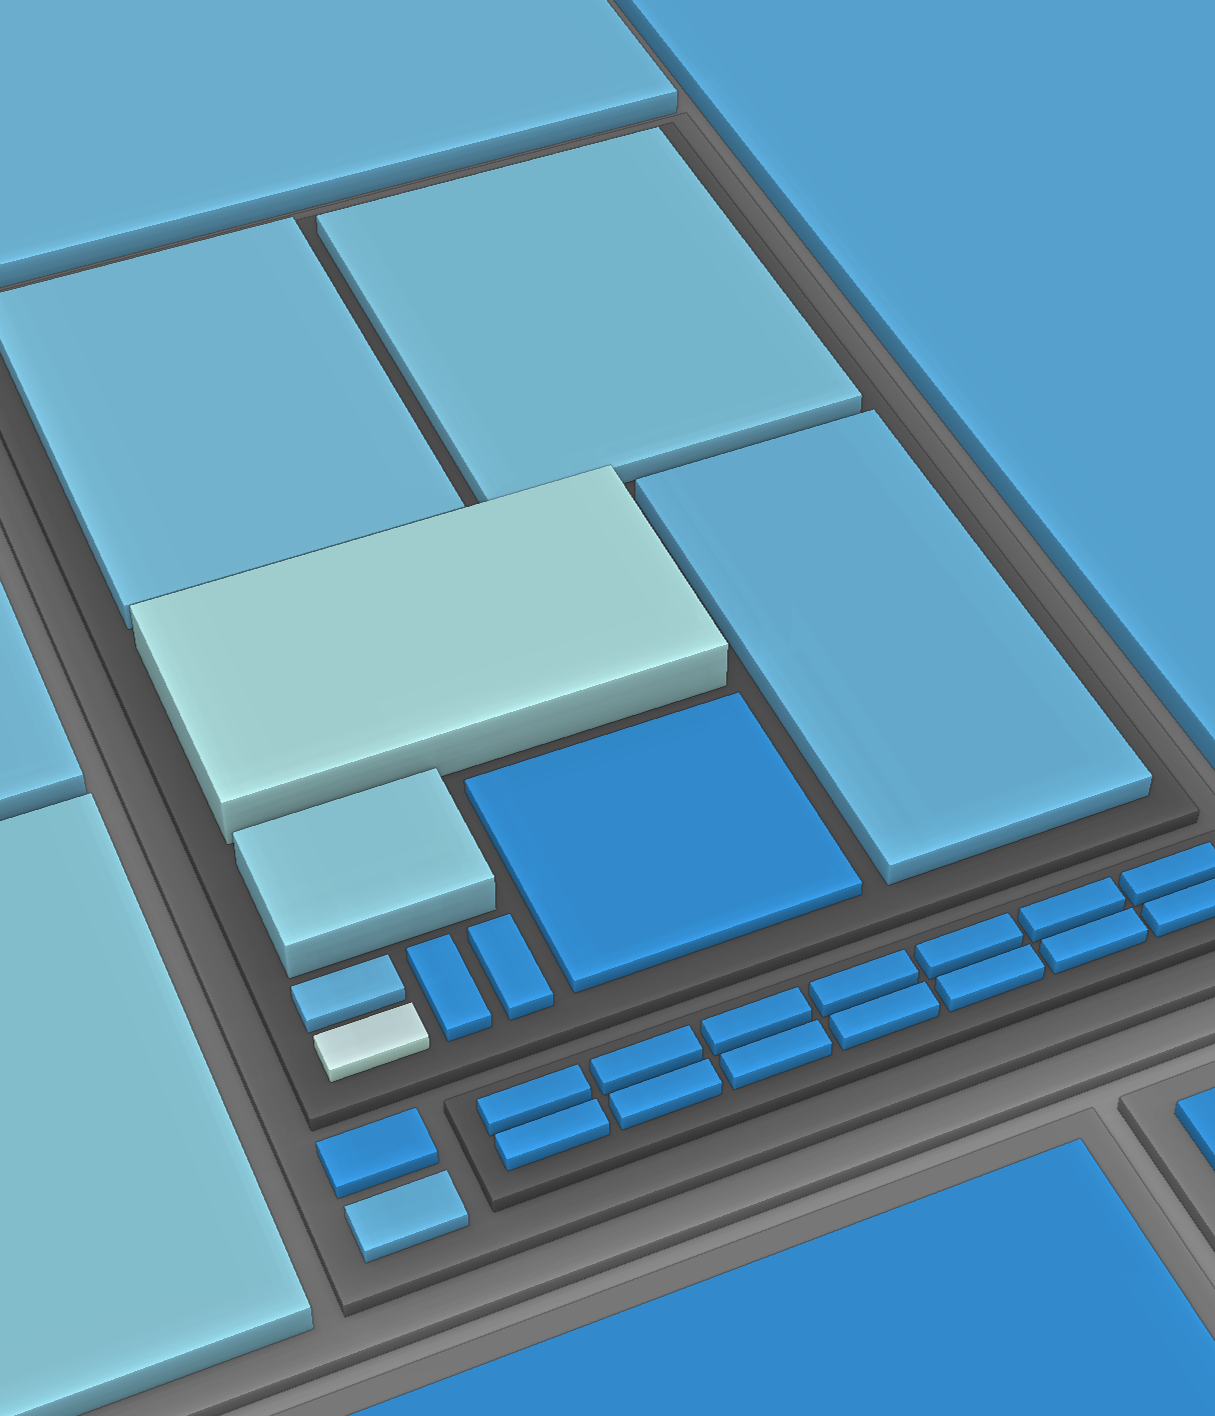
\includegraphics[height=3.5cm]{images/aggregated-1.png}
    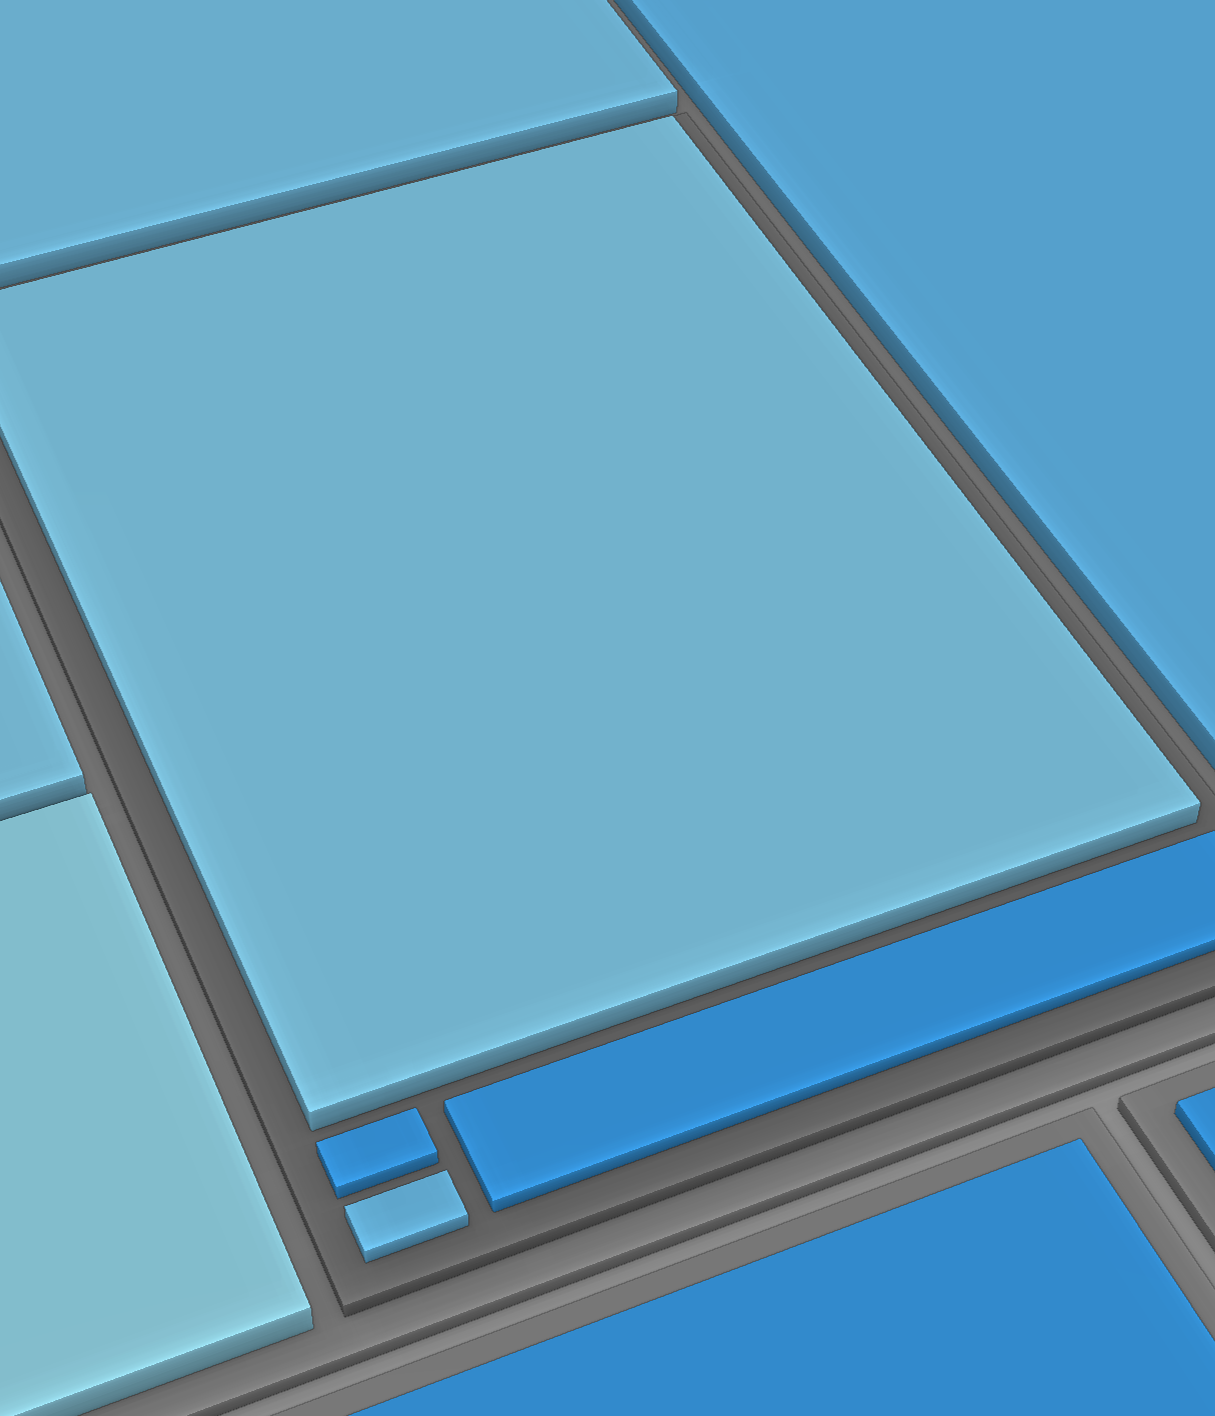
\includegraphics[height=3.5cm]{images/aggregated-2.png}
    \enspace{}\enspace{}
    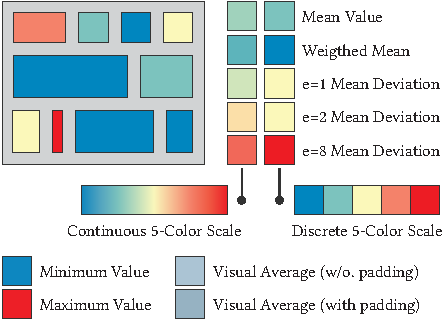
\includegraphics[height=3cm]{images/color-display-v2.pdf}

    \medskip

    Guidelines for hierarchy aggregation (Niklas Elmqvist and Jean-Daniel Fekete, 2009) can be used for identifying and evaluating mitigation strategies:

    \small
    \begin{itemize}
        \item [\textbf{G2}] Visual summary:    \tabto{2.5cm} Aggregates should convey information about underlying data; 
        \item [\textbf{G3}] Visual simplicity: \tabto{2.5cm} Aggregates should be clean and simple; 
        \item [\textbf{G4}] Discriminability:  \tabto{2.5cm} Aggregates should be distinguishable from data items; 
        \item [\ldots] \grayout{Entity Budget, Fidelity, and Interpretability.}
    \end{itemize}

\end{frame} 

\begin{frame}[t]{Depiction of Uncertainty\enspace{}|\enspace{}\textbf{Sketchiness}}

    \smallskip
    \centering
    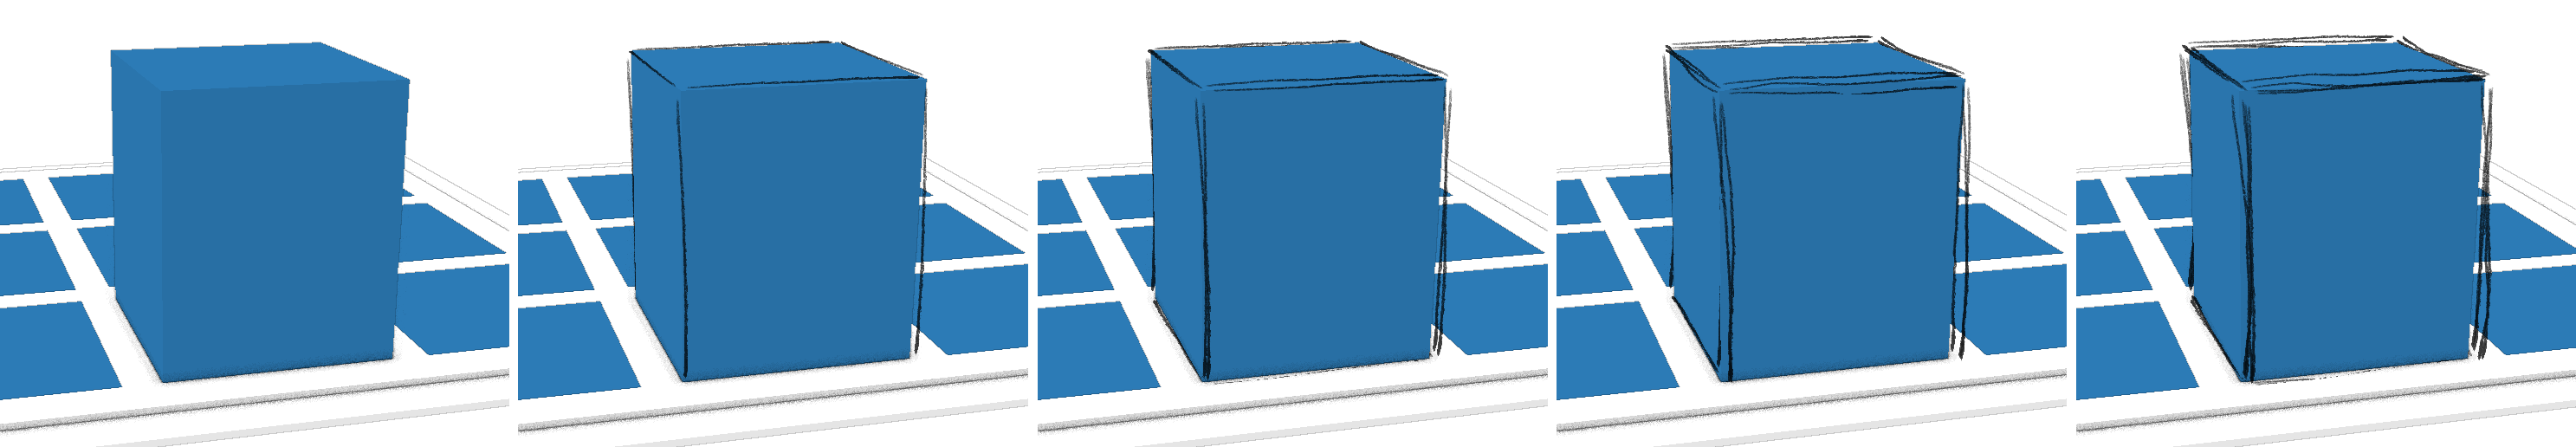
\includegraphics[height=0.25\paperheight]{images/sketchy-scales-biro.png}
    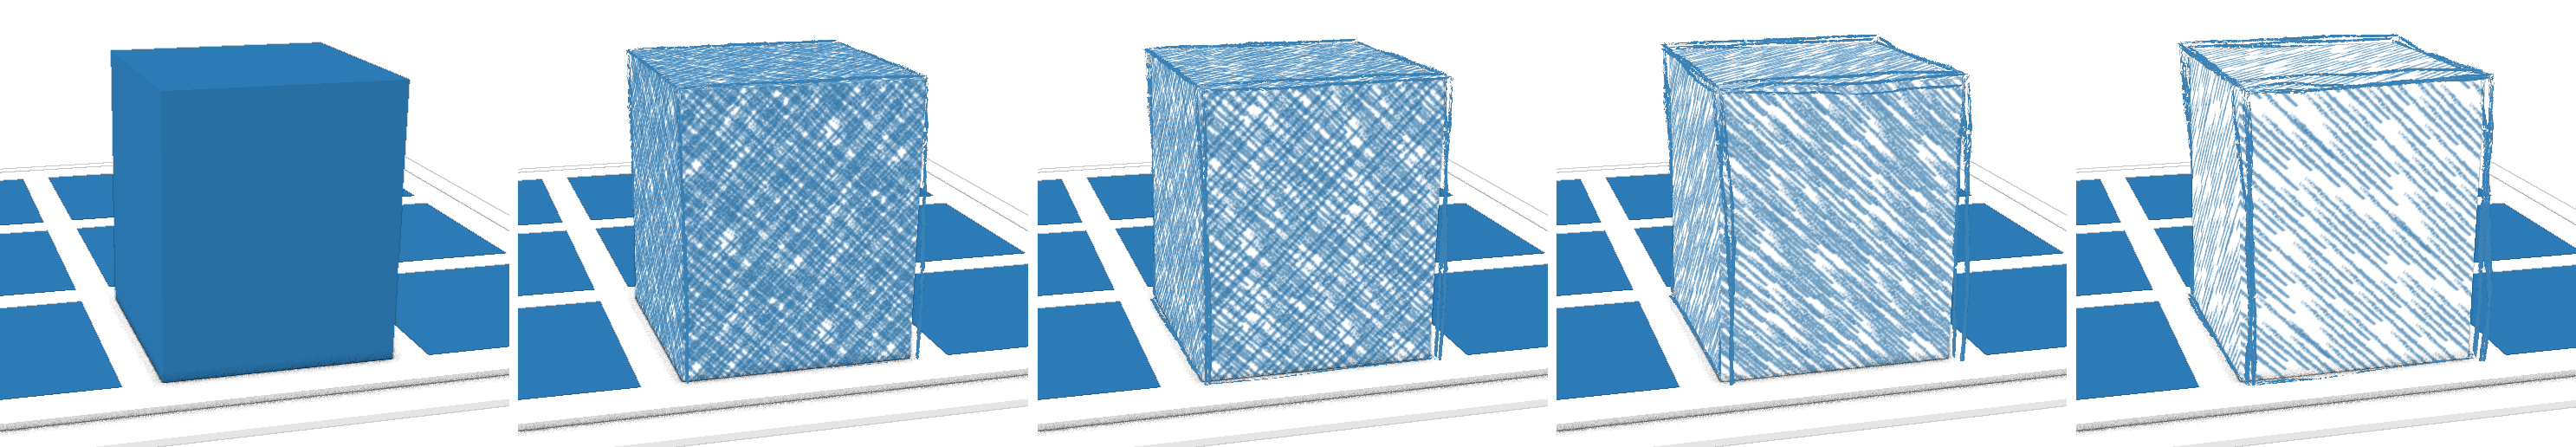
\includegraphics[height=0.25\paperheight]{images/sketchy-scales-pencil.png}
    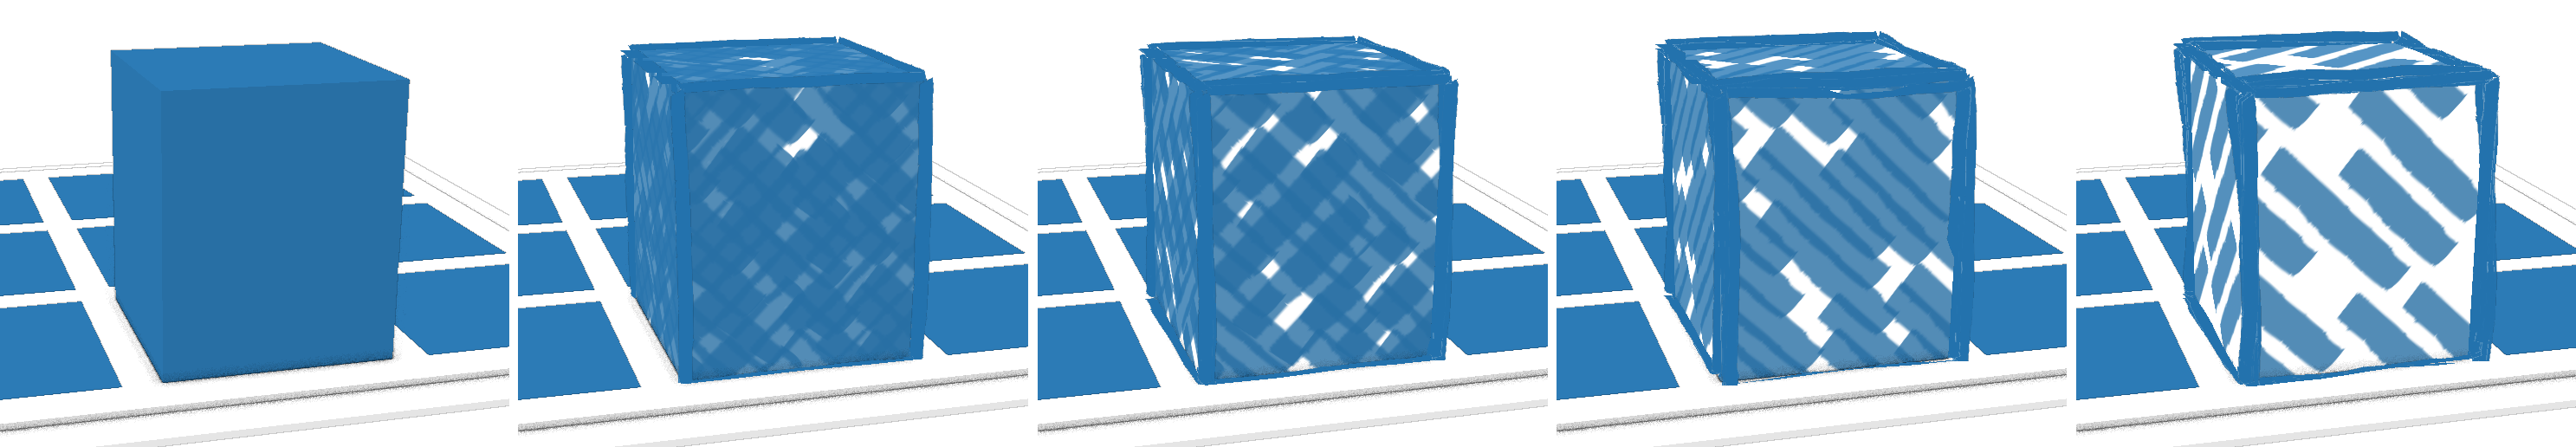
\includegraphics[height=0.25\paperheight]{images/sketchy-scales-marker.png}

\end{frame} 

\begin{frame}[t]{Depiction of Uncertainty\enspace{}|\enspace{}Perlin \textbf{Noise}}

    \smallskip
    \centering
    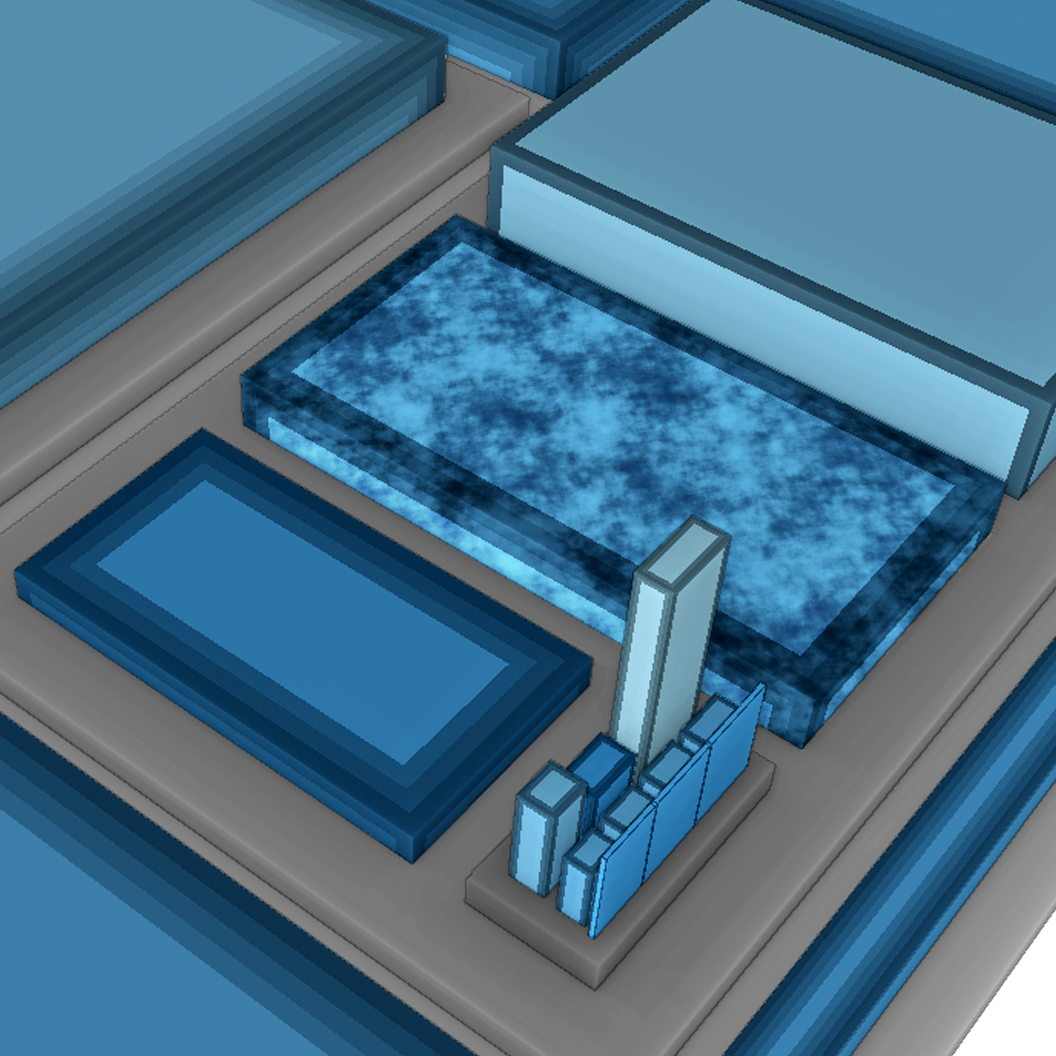
\includegraphics[height=0.75\paperheight, trim=0 32 0 0, clip]{images/aggregation-noise-distribution-a.png}
    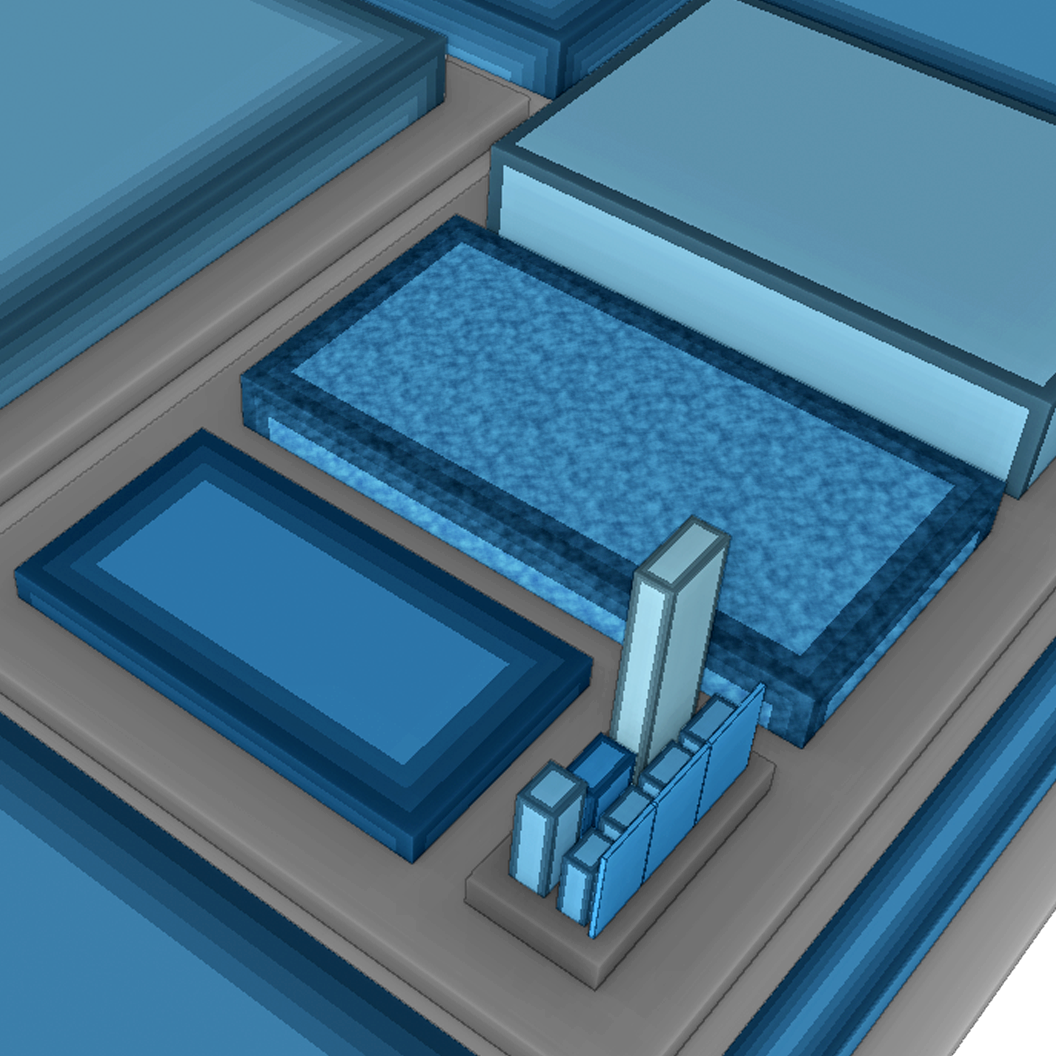
\includegraphics[height=0.75\paperheight, trim=0 32 0 0, clip]{images/aggregation-noise-distribution-b.png}

\end{frame} 

\begin{frame}[t]{Depiction of Uncertainty\enspace{}|\enspace{}\textbf{Color Weaving}}

    \smallskip
    \centering
    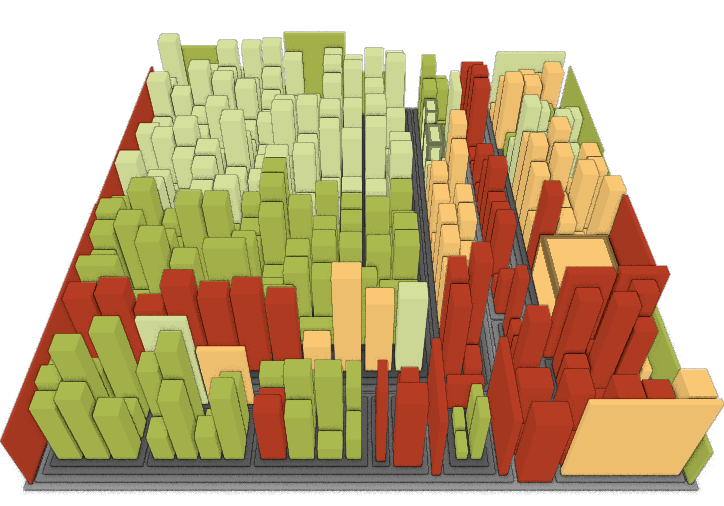
\includegraphics[height=0.75\paperheight, trim=76 0 76 0, clip]{images/color-weaving-4.png}
    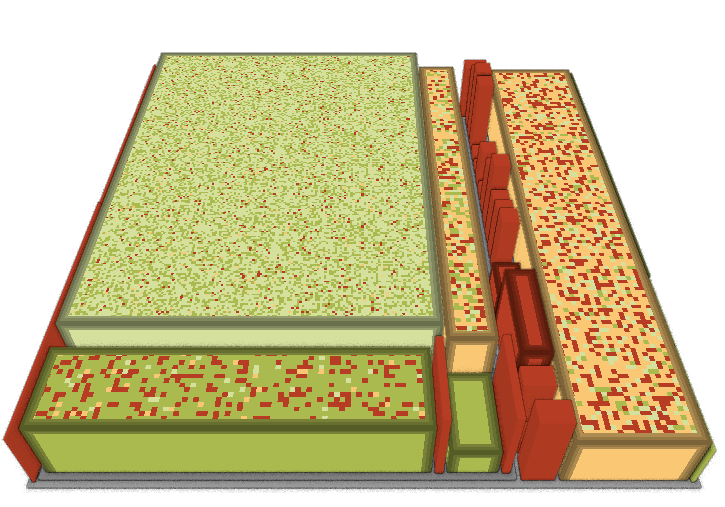
\includegraphics[height=0.75\paperheight, trim=76 0 76 0, clip]{images/color-weaving-3.png}

\end{frame} 

\begin{frame}[t]{Depiction of Uncertainty\enspace{}|\enspace{}\textbf{Color Weaving} \grayout{(area weighted)}}

    \medskip
    \smallskip
    \centering
    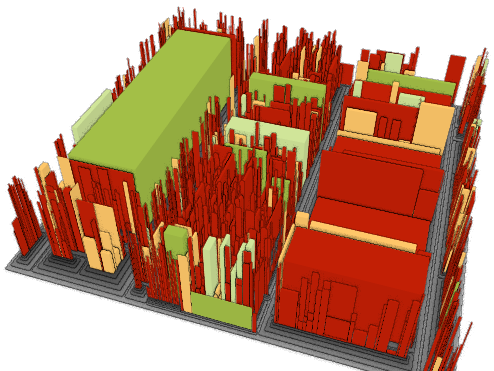
\includegraphics[height=0.75\paperheight, trim=0 0 240 0, clip]{images/teaser-normal-2.png}
    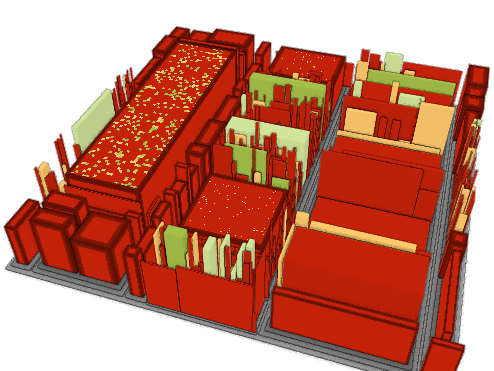
\includegraphics[height=0.75\paperheight, trim=0 0 240 0, clip]{images/teaser-unweighted-2.png}
    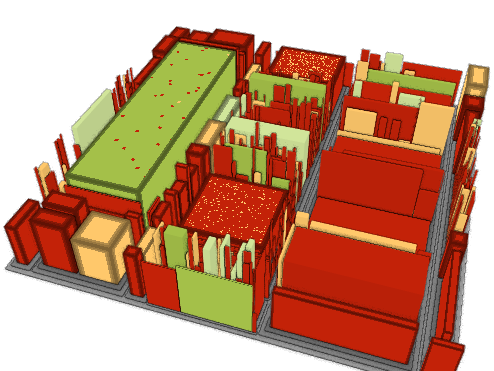
\includegraphics[height=0.75\paperheight, trim=0 0 240 0, clip]{images/teaser-weighted-2.png}

\end{frame} 

\begin{frame}[t]{Depiction of Uncertainty\enspace{}|\enspace{}\textbf{Glyph Charts}}

    \begin{columns}[T,onlytextwidth]

        \column{0.3\textwidth}
        \raggedleft

	    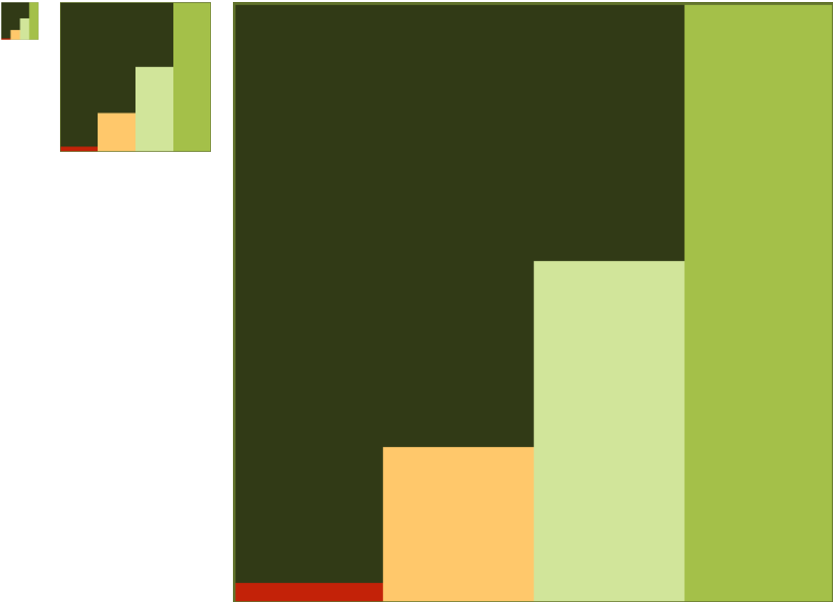
\includegraphics[height=0.184\paperheight]{images/approach-barchart.png}\\
        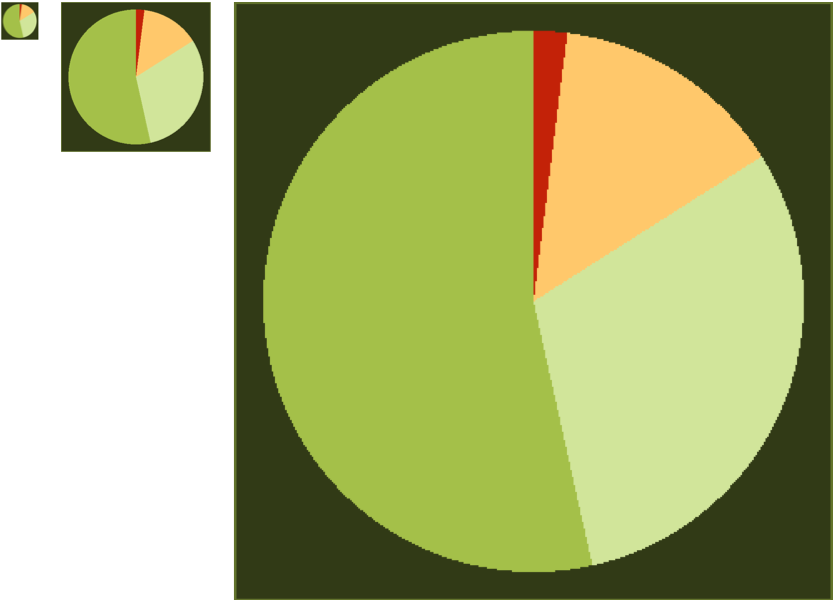
\includegraphics[height=0.184\paperheight]{images/approach-piechart.png}\\
        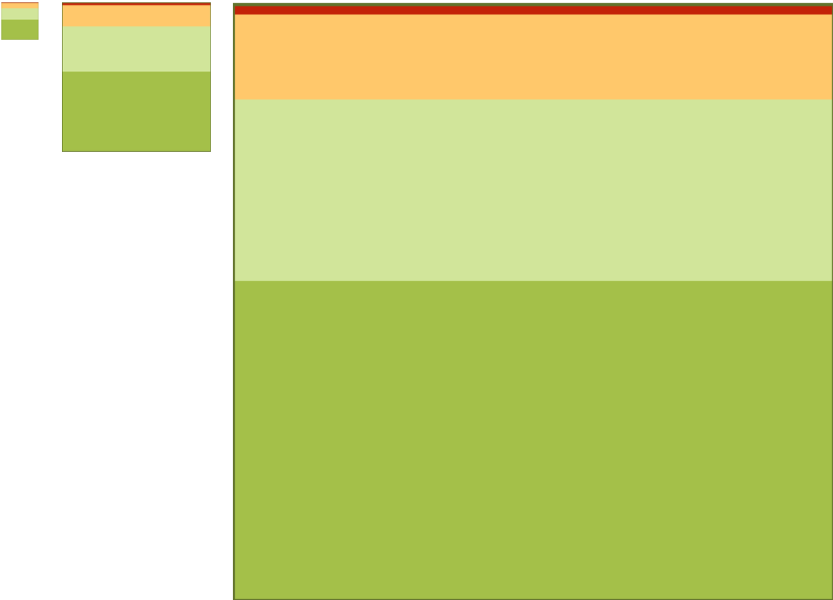
\includegraphics[height=0.184\paperheight]{images/approach-stackedbarchart.png}\\
        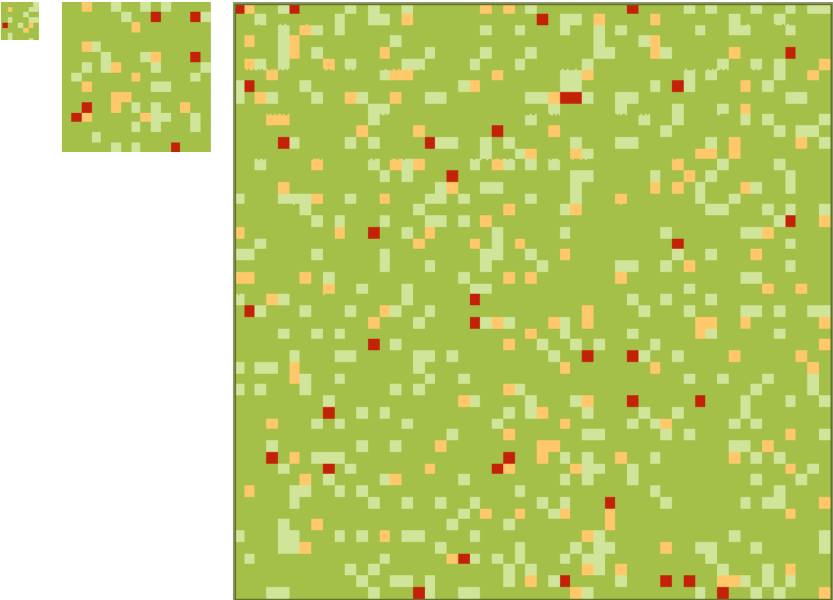
\includegraphics[height=0.184\paperheight]{images/approach-colorweaving.png}

        \column{0.3\textwidth}
        
        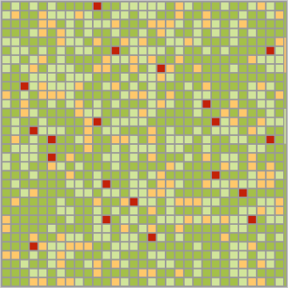
\includegraphics[height=0.75\paperheight]{images/reference.png}

        \column{0.3\textwidth}

    \end{columns}

\end{frame} 

\begin{frame}[t]{Conclusion and Future Work}

    We discussed promising visual variables for superimposition in treemaps to facilitate the visual display of uncertainty in mapped attributes and aggregated/underlying value distributions.

    \bigskip

    \textbf{Perceptual Questions}:
    \begin{itemize}
        \item Color Weaving: what underlying distribution is expected w.r.t. area, size, and number of outliers.
        \item Which glyph are best suited (can be read most accurately) for small display. 
        \item To what extent can sketchiness be superimposed to color without reducing its accuracy.
    \end{itemize}
    \medskip
    
    \textbf{Technical Challenges}:
    \begin{itemize}
        \item Glyph placement and adaptive glyph scaling.
        \item Adaptive size computation for minimal representative patches for color weaving.
    \end{itemize}
    \bigskip
    
    For questions, exchange of ideas, and collaboration contact us at \{daniel.limberger,matthias.trapp,juergen.doellner\}@hpi.de

\end{frame} 

\end{document}

